\documentclass[peerreview]{IEEEtran}
\usepackage{cite} % Tidies up citation numbers.
\usepackage{url} % Provides better formatting of URLs.
\usepackage[utf8]{inputenc} % Allows Turkish characters.
\usepackage{booktabs} % Allows the use of \toprule, \midrule and \bottomrule in tables for horizontal lines
\usepackage{graphicx}
\usepackage{xcolor}
\usepackage{subcaption} % For subfigures
\usepackage{hyperref}
\usepackage{subcaption}
\usepackage{amsmath}

\hyphenation{op-tical net-works semi-conduc-tor} % Corrects some bad hyphenation 

\begin{document}
%\begin{titlepage}
% paper title
% can use linebreaks \\ within to get better formatting as desired
\title{Machine Learning in Applications \\ AM03 Project Report}

% author names and affiliations

\author{Barbieri Fabio, Di Giorgio Vittorio, Ferrigno Antonio, Scoleri Maria Rosa\\
Politecnico di Torino\\
}
\date{24/07/2024}

% make the title area
\maketitle
\tableofcontents
\newpage
\listoffigures
\listoftables
%\end{titlepage}

\IEEEpeerreviewmaketitle
\begin{abstract}
This study evaluates the efficacy of different self-supervised learning (SSL) methods for feature extraction from a Colorectal Cancer Whole Slide Images dataset (CRC-WSIs). We compare these SSL approaches against conventional transfer learning techniques using ImageNet pre-trained Convolutional Neural Networks (CNNs). To ensure a fair and straightforward comparison, we assess each model's representational capabilities by using their learned embeddings as input to a linear SVM for a cancer detection task. Our investigation involves a representative set of SSL methods, including state-of-the-art architectures, training strategies, and data augmentation techniques. The selected methods include a Variational Autoencoder, a rotation agnostic framework that includes Vision Transformers (PathDino), and a contrastive learning method (Bootstrap Your Own Latent, BYOL). 
We find that PathDino, especially when fine-tuned, outperforms the other models in extracting meaningful features. Interesting results are given by BYOL as well, prompting an interesting discussion on the augmentation techniques for medical images.

\vspace{0.2cm} 
\noindent For more information and code, please visit  \href{https://github.com/s316467/ML-in-Apps-2024-AM03-Extracting-Features-from-Medical-Images}{our GitHub repository}.
\end{abstract}



\section{Introduction}
\label{sec:introduction}
The digital pathology field has greatly benefited from the advancements in Deep Learning in recent years, particularly in the application of deep learning models for analyzing Whole Slide Images (WSIs). These high-resolution images provide a high amount of information for diagnosing and studying diseases such as colorectal cancer (CRC). However, effective use of deep learning models in this domain faces several challenges, including the scarcity of large-scale annotated datasets and the high computational resources required.

Traditional approaches have relied heavily on transfer learning, where models pre-trained on large natural image datasets like ImageNet\cite{imagenet} are fine-tuned for specific pathology tasks. While this method has shown promise, it raises questions about the appropriateness of using features learned from natural images for medical imaging tasks, given the significant domain differences. Self-supervised learning (SSL) has emerged as a powerful alternative, offering the potential to learn meaningful representations from unlabeled medical imaging data. SSL methods can leverage the vast amounts of unlabeled WSIs available in pathology archives, potentially capturing domain-specific features more relevant to pathology tasks than those learned from natural images\cite{survey}. However, the applicability of typical SSL augmentation techniques to WSIs is problematic. Many SSL methods rely on augmentations such as rotations, flips, blurs, and color jittering, which are effective for natural images but may not be appropriate or beneficial for histopathological images. For instance, blurring can make it difficult to clearly see the size, shape, and chromatin pattern of tumor cell nuclei. The orientation of tissue structures may carry diagnostic significance, so arbitrary rotations could potentially distort important features. Similarly, color variations in histopathology images are often meaningful and tied to staining processes, making indiscriminate color augmentations potentially counterproductive. These concerns highlight the need for a careful evaluation of SSL methods and their augmentation strategies in the context of WSIs.

The purpose of this study is to conduct a comprehensive evaluation of various SSL methods for feature extraction from Colorectal Cancer Whole Slide Images (CRC-WSIs), comparing their efficacy against conventional transfer learning approaches. By focusing on a diverse set of SSL techniques, including Variational Autoencoders (VAEs\cite{vae}), rotation-agnostic frameworks with Vision Transformers (PathDino\cite{pathdino}), and contrastive learning methods like Bootstrap Your Own Latent (BYOL\cite{byol}), we aim to provide insights into the most effective approaches for learning representations from WSIs. Our investigation is designed to address several key questions: How do different SSL methods compare in their ability to extract meaningful features from CRC-WSIs? How do the relative performances relate to model training strategies and architectures? Can SSL approaches outperform traditional transfer learning techniques using ImageNet pre-trained Convolutional Neural Networks (CNNs) in the context of digital pathology?

To ensure a fair and interpretable comparison, we evaluate these methods by using their learned embeddings as input to a linear Support Vector Machine (SVM) for a cancer detection task. This approach allows us to assess the quality of the learned representations directly, without employing complex downstream architectures. %

\begin{figure*}
    \centering
    \begin{subfigure}[b]{0.36\textwidth}
        \centering
        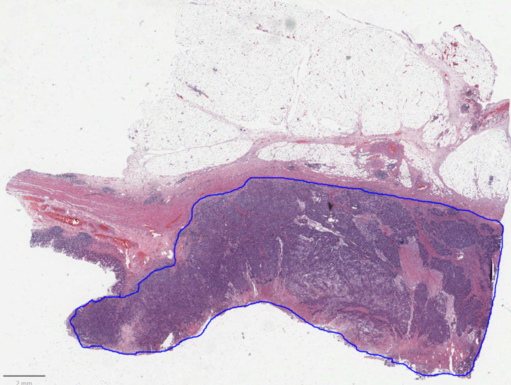
\includegraphics[width=\textwidth]{figure/1svs.png}
        \caption{Original WSI image}
        \label{fig:1svs}
    \end{subfigure}
    \hfill
    \begin{subfigure}[b]{0.26\textwidth}
        \centering
        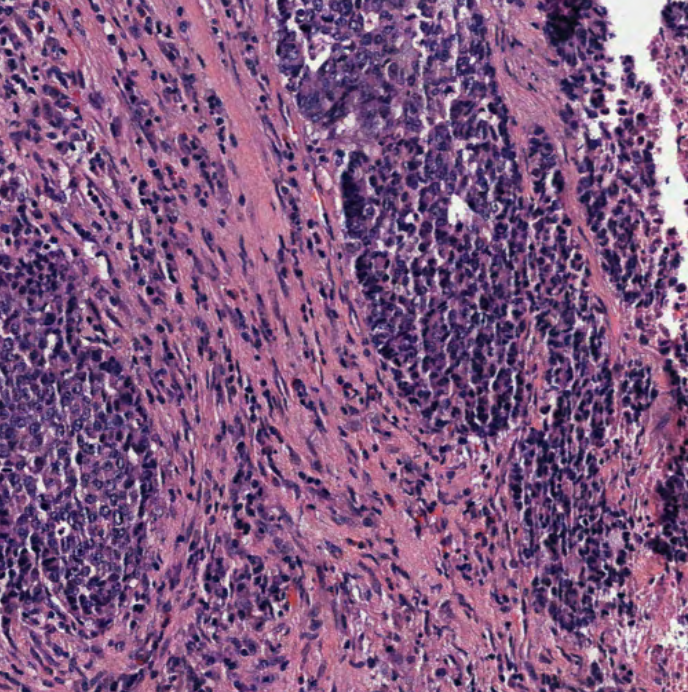
\includegraphics[width=\textwidth]{figure/cpatch.png}
        \caption{Cancerous patch}
        \label{fig:ncpatch}
    \end{subfigure}
    \hfill
    \begin{subfigure}[b]{0.26\textwidth}
        \centering
        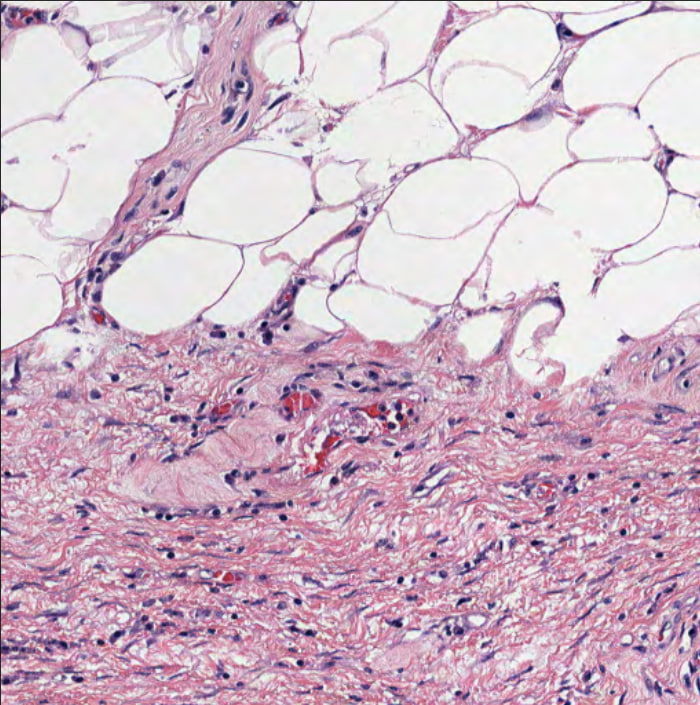
\includegraphics[width=\textwidth]{figure/ncpatch.jpg}
        \caption{Non-cancerous patch}
        \label{fig:cpatch}
    \end{subfigure}
    \caption{\small Figure (a) shows an example of a WSI image taken from the CRC-WSIs dataset. The blue border delimits the cancerous region of the image. (b) represents a cancerous patch taken from the inside of the blue border of the original image, and (c) shows a non-cancerous patch.}
    \label{fig:wsiexample}
\end{figure*}

\section{Background}
Representation learning has become a cornerstone in medical imaging, especially in relation to its application to digital pathology. Over the years, several methods have been developed and tested in this field, including techniques of unsupervised learning and self-supervised learning.

Variational Autoencoders (VAEs) have emerged as a powerful tool in the field of representation learning for medical imaging. For example, the work presented in \cite{breastcancer} exploits the encoding of VAEs to analyze histopathological images resulting from breast tissue biopsies to classify the tumor as cancerous or benign. The research presented in \cite{Nasr_2023} introduces a VAE-based approach to compress and decompress cancer pathology slides verifying that the compression still allows to maintain accuracy in clinical validation tasks. The same conclusion can be found in \cite{digpat}.
VAEs, however, are not without limitations: in some scenarios, they struggle to represent fine details or sharp transitions in the data, this is why more advanced methods have also been developed.

A recent advancement in the representation learning of medical images is the use of models based on Vision Transformer (ViT) \cite{vit}. Thanks to the attention mechanism \cite{attention}, transformers have proven to be capable of learning long-range dependencies and spatial correlations both in Natural Language Processing and in Computer Vision. The review presented in \cite{reviewvit} shows how ViTs are used in different medical image analysis tasks, including classification, segmentation, detection, and clinical report generation. ViTs however, can fail to account for the unique characteristics of histopathological images. They also require large amounts of data to perform optimally and can face issues of overfitting. To address these challenges, the authors of \cite{pathdino} present a model called \textbf{PathDino}, which is a new ViT-based approach that is designed specifically for histopathological images. PathDino is a lightweight and compact feature extractor built with five transformer blocks. Accompanied by a novel patch selection method and a rotation augmentation technique, PathDino demonstrates superior performance and effectively manages to reduce overfitting. This work is particularly relevant to our study and will be further analyzed and tested in relation to our dataset.

To further enhance the quality of learned representations in medical images, contrastive learning models have also been explored. The work presented in \cite{contrglobloc}, for example, proposes different strategies for extending the contrastive learning framework for the segmentation of volumetric medical images with limited
annotation. The authors of \cite{contr2} highlight the need to develop a method capable of learning effective representations when labeled data are scarce, and they introduce novel contrasting strategies that leverage structural similarity across volumetric medical images. 


\begin{figure*}
\centering
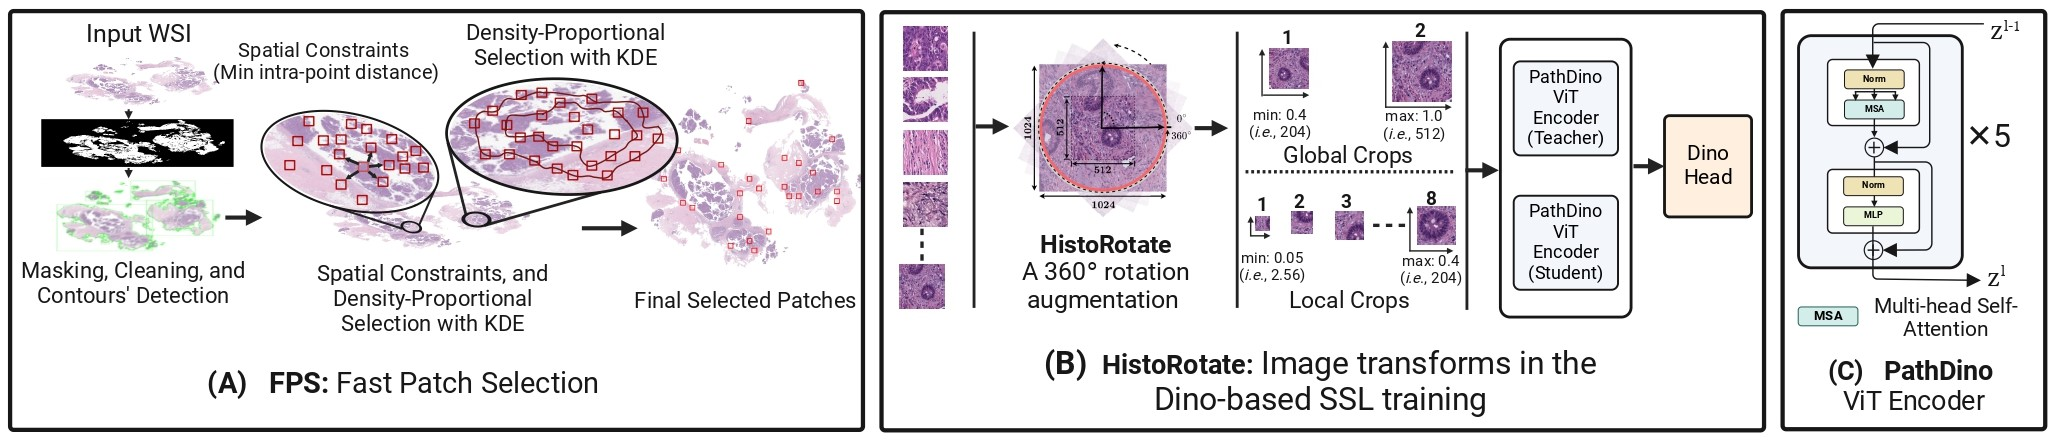
\includegraphics[width=\textwidth]{figure/PathDino2.jpg} 
\caption[The WSI Analysis Pipeline]{\small The figure shows the WSI Analysis Pipeline and it is taken from \cite{pathdino}. (A) The Fast Patch Selection (FPS) method chooses a group of representative patches while maintaining their spatial arrangement. (B) HistoRotate is a 360\textdegree rotation augmentation for histopathology model training that helps the representations of the models become rotation invariant. (C) PathDino is a compact histopathology Transformer with five small vision transformer blocks and about 9 million parameters}
\label{fig:PathDino}
\end{figure*}


%todo: all methods descriptions: shouldn't we mention why we choose them in relationship to WSI?%
\section{Materials and Methods}
\label{sec:methods}
In this section, we provide a comprehensive description of the materials and methodologies used in our investigation. Starting with the dataset description and the extracted patches, moving forward to the baselines, and finally to the self-supervised learning methods we tested.

\subsection{Dataset}
Our study focuses on a set of Colorectal Cancer Whole Slide Images (CRC-WSIs) from 24 patients. Each patient's data consists of an SVS image and a corresponding XML file containing Region-of-Interest (ROI) coordinates which delineate areas of cancer presence. To create a suitable dataset, we processed the images to extract 512x512 pixel patches at magnification level 1 - which has a 0.252 downsampling factor. The extracted patches are then further processed to obtain a dataset of (patch, label) pairs where labels are boolean values encoding cancer presence in the relative patch. We used the Ray Casting algorithm as a labeling method in order to determine if patch vertices fall within the cancerous region. An example of a WSI image and patches taken from our dataset is shown in Figure \ref{fig:wsiexample}.
The obtained dataset has the following characteristics:
\begin{itemize}
    \item Total samples: 13878
    \item Cancerous samples: 6880
    \item Non-cancerous samples: 6998
\end{itemize} As we can see the obtained dataset is fairly balanced, but it is relatively small compared to typical WSI settings (\cite{ehteshami2017diagnostic
}), emphasizing the need for suitable augmentation techniques.

\subsection{Baselines}
The baselines chosen to test the strength of SSL methods are the DenseNet121\cite{densenet} and ResNet50\cite{resnet} networks. 

DenseNet-based models have been used extensively in the field of medical imaging for tasks such as classification \cite{CHAUHAN2021100020, densetcovid}, pattern recognition, image segmentation, and object detection \cite{densetmedanalysis}. We selected DenseNet121 as a baseline model due to its strong representational capabilities while being less computationally expensive compared to deeper architectures. For this study, we use the DenseNet121 model pre-trained on ImageNet, and no specific hyperparameter tuning was performed. 

ResNet50\cite{resnet} is another widely used CNN architecture that is deeper than DenseNet121, consisting of 50 layers. It is built on the concept of residual learning, where shortcut connections, or "skip connections," allow for the construction of very deep networks by alleviating the vanishing gradient problem. In the context of digital pathology, ResNet50's deep architecture and efficient learning mechanism make it particularly well-suited for capturing the intricate patterns and multi-scale features present in Whole Slide Images. Its proven track record in transfer learning scenarios, where models pre-trained on large datasets like ImageNet are adapted to specific medical imaging tasks, further justifies its selection as a strong baseline for our comparative study\cite{tlsurvey}.


\subsection{BYOL}
Bootstrap Your Own Latent (BYOL) is a self-supervised learning framework that learns image representations without the need for negative pairs, differing from traditional contrastive learning methods. BYOL employs two neural networks, an online network and a target network, which learn collaboratively via a bootstrapping mechanism. The online network comprises an encoder, a projector, and a predictor, which process input images to produce embeddings that are aligned with the outputs of the target network. The target network, which does not include a predictor, shares a similar architecture but updates its parameters as a moving average of the online network's parameters, allowing for gradual evolution. The core of BYOL's learning mechanism is its loss function, which aims to align the outputs of the predictor in the online network with the target network. Given two augmented views of an image, $v$ and $v'$, the loss function is defined as:
\[
\mathcal{L}_{BYOL} = 2 - 2 \cdot \frac{\langle q_{\theta}(z_{\theta}), z'_{\xi} \rangle}{\|q_{\theta}(z_{\theta})\|_2 \cdot \|z'_{\xi}\|_2}.
\]
In this loss function:
\begin{itemize}
    \item $q_{\theta}(z_{\theta})$ is the output of the predictor network in the online network.
    \item $z'_{\xi}$ is the embedding generated by the target network from an augmented view $v'$ of the input image.
    \item $\langle q_{\theta}(z_{\theta}), z'_{\xi} \rangle$ denotes the dot product between the predictor's output and the target network's embedding.
    \item $\|q_{\theta}(z_{\theta})\|_2$ and $\|z'_{\xi}\|_2$ are the L2 norms of the vectors $q_{\theta}(z_{\theta})$ and $z'_{\xi}$, respectively.
\end{itemize}
This loss measures the cosine similarity between the normalized outputs of the online network's predictor and the target network, promoting similarity between representations of different augmented views of the same image. To avoid representation collapse, where the model produces identical outputs for all inputs, BYOL uses an asymmetric design. The target network serves as a stable reference with slowly evolving parameters, while the predictor in the online network drives the learning of diverse and meaningful features, preventing convergence to trivial solutions.


\begin{figure*}
\centering
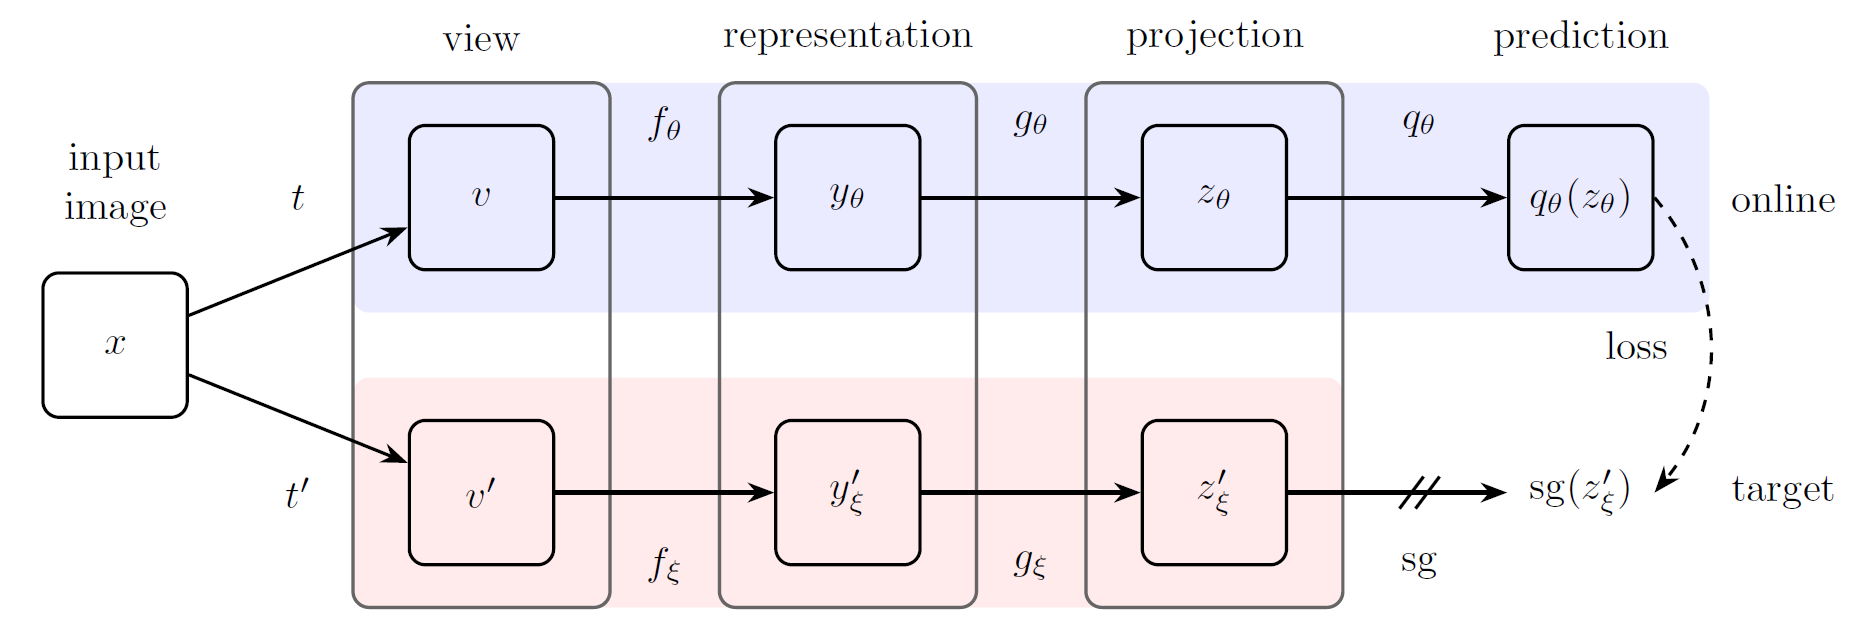
\includegraphics[width=0.8\textwidth]{figure/BYOL.png} 
\caption{\small BYOL Architecture from \cite{byol}. BYOL minimizes a similarity loss between the prediction part of the online network $q_{\theta}(z_{\theta})$ and the output of the target network after stop gradient $sg(z^{'}_\xi)$. $\theta$ symbolizes the trained weights and $\xi$ are an exponential moving average of $\theta$. After training, everything except $f_\theta$ is discarded and $y_\theta$ is used as the image representation. }
\label{fig:BYOL}
\end{figure*}

\subsection{PathDino}
PathDino is a self-supervised learning model specifically designed to enhance image representation learning in digital pathology. A schematic representation of the model's architecture and process can be found in Figure \ref{fig:PathDino}. It employs a compact transformer-based architecture with approximately 9 million parameters, making it efficient for deployment in systems with limited computational resources. PathDino's framework includes an architecture with five small vision transformer blocks, a Fast Patch Selection (FPS) method, and a rotation augmentation technique called HistoRotate.

Key Components are:
\begin{itemize}
    \item \textbf{Fast Patch Selection (FPS):} Selects representative patches from whole slide images (WSIs) while preserving spatial distribution. The process consists of creating a smaller thumbnail image from the WSI, as well as a tissue mark to identify areas of interest. Potential patch locations are determined based on contours in the tissue mark. Then, Kernel Density Estimation (KDE) is used to calculate the density of these potential patches and select them. A minimum distance is maintained between selected patches to avoid choosing too many patches from densely packed regions. Finally, the selected patches are mapped back to their original positions in the high-resolution WSI.
    \item \textbf{HistoRotate:} A 360-degree rotation augmentation method that enhances learning without altering the contextual information of histopathology images. Two rotations are considered: an angle is sampled from a continuous uniform distribution in the range $[0,360]$ degrees. A second discrete rotation is selected from the set $\Theta=\{90,180,270,360\}$.
    \item \textbf{Vision Transformer Blocks:} The model architecture is composed of five compact Vision Transformers blocks. Each block is made with a multi-head self-attention (MSA) layer, Layer Norm (LN), and a Multilayer Perceptron (MLP):
    \begin{equation}
        \textbf{z}^l_i = MLP(LN(MSA(\textbf{z}^{l-1}_i))) + \textbf{z}^{l-1}_i
    \end{equation}
    where  $l=1,...,L$ and $n=1,...,N$ with $L=5$ blocks and $N$ represents the total input patches.
\end{itemize}

The attention mechanism in PathDino plays a crucial role in capturing critical features from histopathology images by focusing on different regions of the input image through multiple attention heads. Each of the five attention heads in PathDino's vision transformer model generates an attention map that highlights distinct tissue structures and patterns. Figure \ref{fig:attention_pathdino} illustrates the attention maps generated by each head.


\begin{figure}
\centering
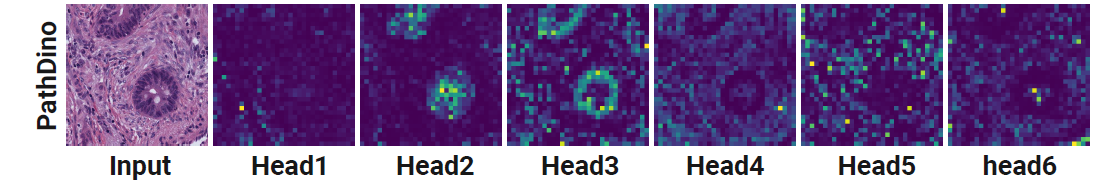
\includegraphics[width=\columnwidth]{figure/attention_pathdino.png} 
\caption[Pathdino Attention Layers Visualization.]{\small Visualization of attention maps generated by different attention heads in the PathDino model \cite{b5}. The input histopathology image is shown on the left, followed by the attention maps from each of the six attention heads. These maps illustrate how each head in the transformer model focuses on different elements of the tissue structure, highlighting the model's ability to capture critical features across multiple levels of abstraction in the input image.} 

\label{fig:attention_pathdino}
\end{figure}



\subsection{ResVAE}
Variational Autoencoders \cite{vae} have proved to be one of the most effective tools for representation learning. For the purpose of our work we employ a variational autoencoder based on a ResNet \cite{resnet} architecture (ResVAE)
\footnote{
    The implementation of the variational autoencoder is strongly inspired by the work in \href{https://github.com/julianstastny/VAE-ResNet18-PyTorch}{this} folder.
}. In particular, the encoder is a modified version of a ResNet18 in which the series of residual blocks with skip connections performs the downscaling of the image. The decoder is a mirror of the encoder and performs the upscaling operation.
The VAE employs the reparameterization trick to sample from the latent space during training, utilizes a Mean-Squared Error (MSE) as reconstruction loss, and the KL Divergence to regularize the latent space. The MSE and the KL divergence can be formalized as follows:
\begin{equation}
    \text{MSE}= \frac{1}{n} \sum_{i=1}^n (x_i - \hat{x}_i)^2
\end{equation}
\begin{equation}
    \text{KL}(q(z|x)||p(z))=\frac{1}{2} \sum_{j=1}^d (1+log(\sigma_j^2)-\mu_j^2-\sigma_j^2)
\end{equation}
where
\begin{itemize}
    \item $q(z|x)$ represents the learned latent distribution
    \item $p(z)$ is the target distribution, usually a standard normal distribution
    \item $1+log(\sigma_j^2)$ is the term that penalizes the model if the variance $\sigma_j^2$ deviates from 1
    \item $\mu_j^2$ penalizes the model for having a mean $\mu$ that deviates from 0
    \item $\sigma_j^2$ encourages the variance to be close to 1
\end{itemize}
VAEs require a careful balance between these two losses in order to achieve better performance: minimizing more the reconstruction loss may lead to overfitting but minimizing more the KL divergence could mean that the model does not learn effectively enough the distribution of the training data

\subsection{SVM training}
The embeddings extracted from all the aforementioned models are then fed to a linear Support Vector Machine (SVM), which is trained to classify each image as cancerous or non-cancerous.
The performance of the SVM reflects the ability of the chosen models to correctly represent the input images and retain the information useful to identify cancerogenous tissue. The SVM was chosen for its simplicity and strong performance in high-dimensional spaces. It is important to underline that all the models presented are trained in a self-supervised manner and used as features extractors. The SVM is the only model that has access to the labeled images. t-Distributed Stochastic Neighbor Embedding (t-SNE) was applied to the PCA-reduced features for visualization. A scatter plot was generated to visualize the clustering of predicted labels in a 2D space, providing insight into the classifier's performance.

\section{Results and Discussion}
\begin{figure*}[ht]
    \centering
    \begin{subfigure}[b]{0.3\textwidth}
        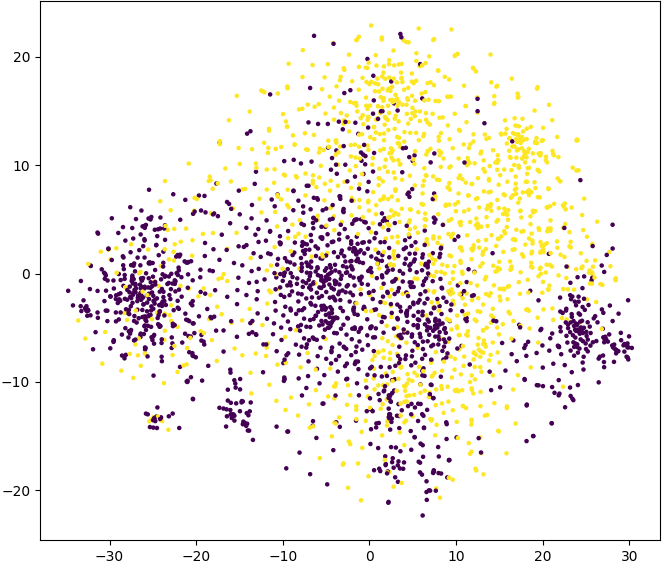
\includegraphics[width=\textwidth]{figure/Densenet121_tsne.png}
        \caption{Densenet121}
        \label{fig:tsne_densenet}
    \end{subfigure}
    \hfill
    \begin{subfigure}[b]{0.3\textwidth}
        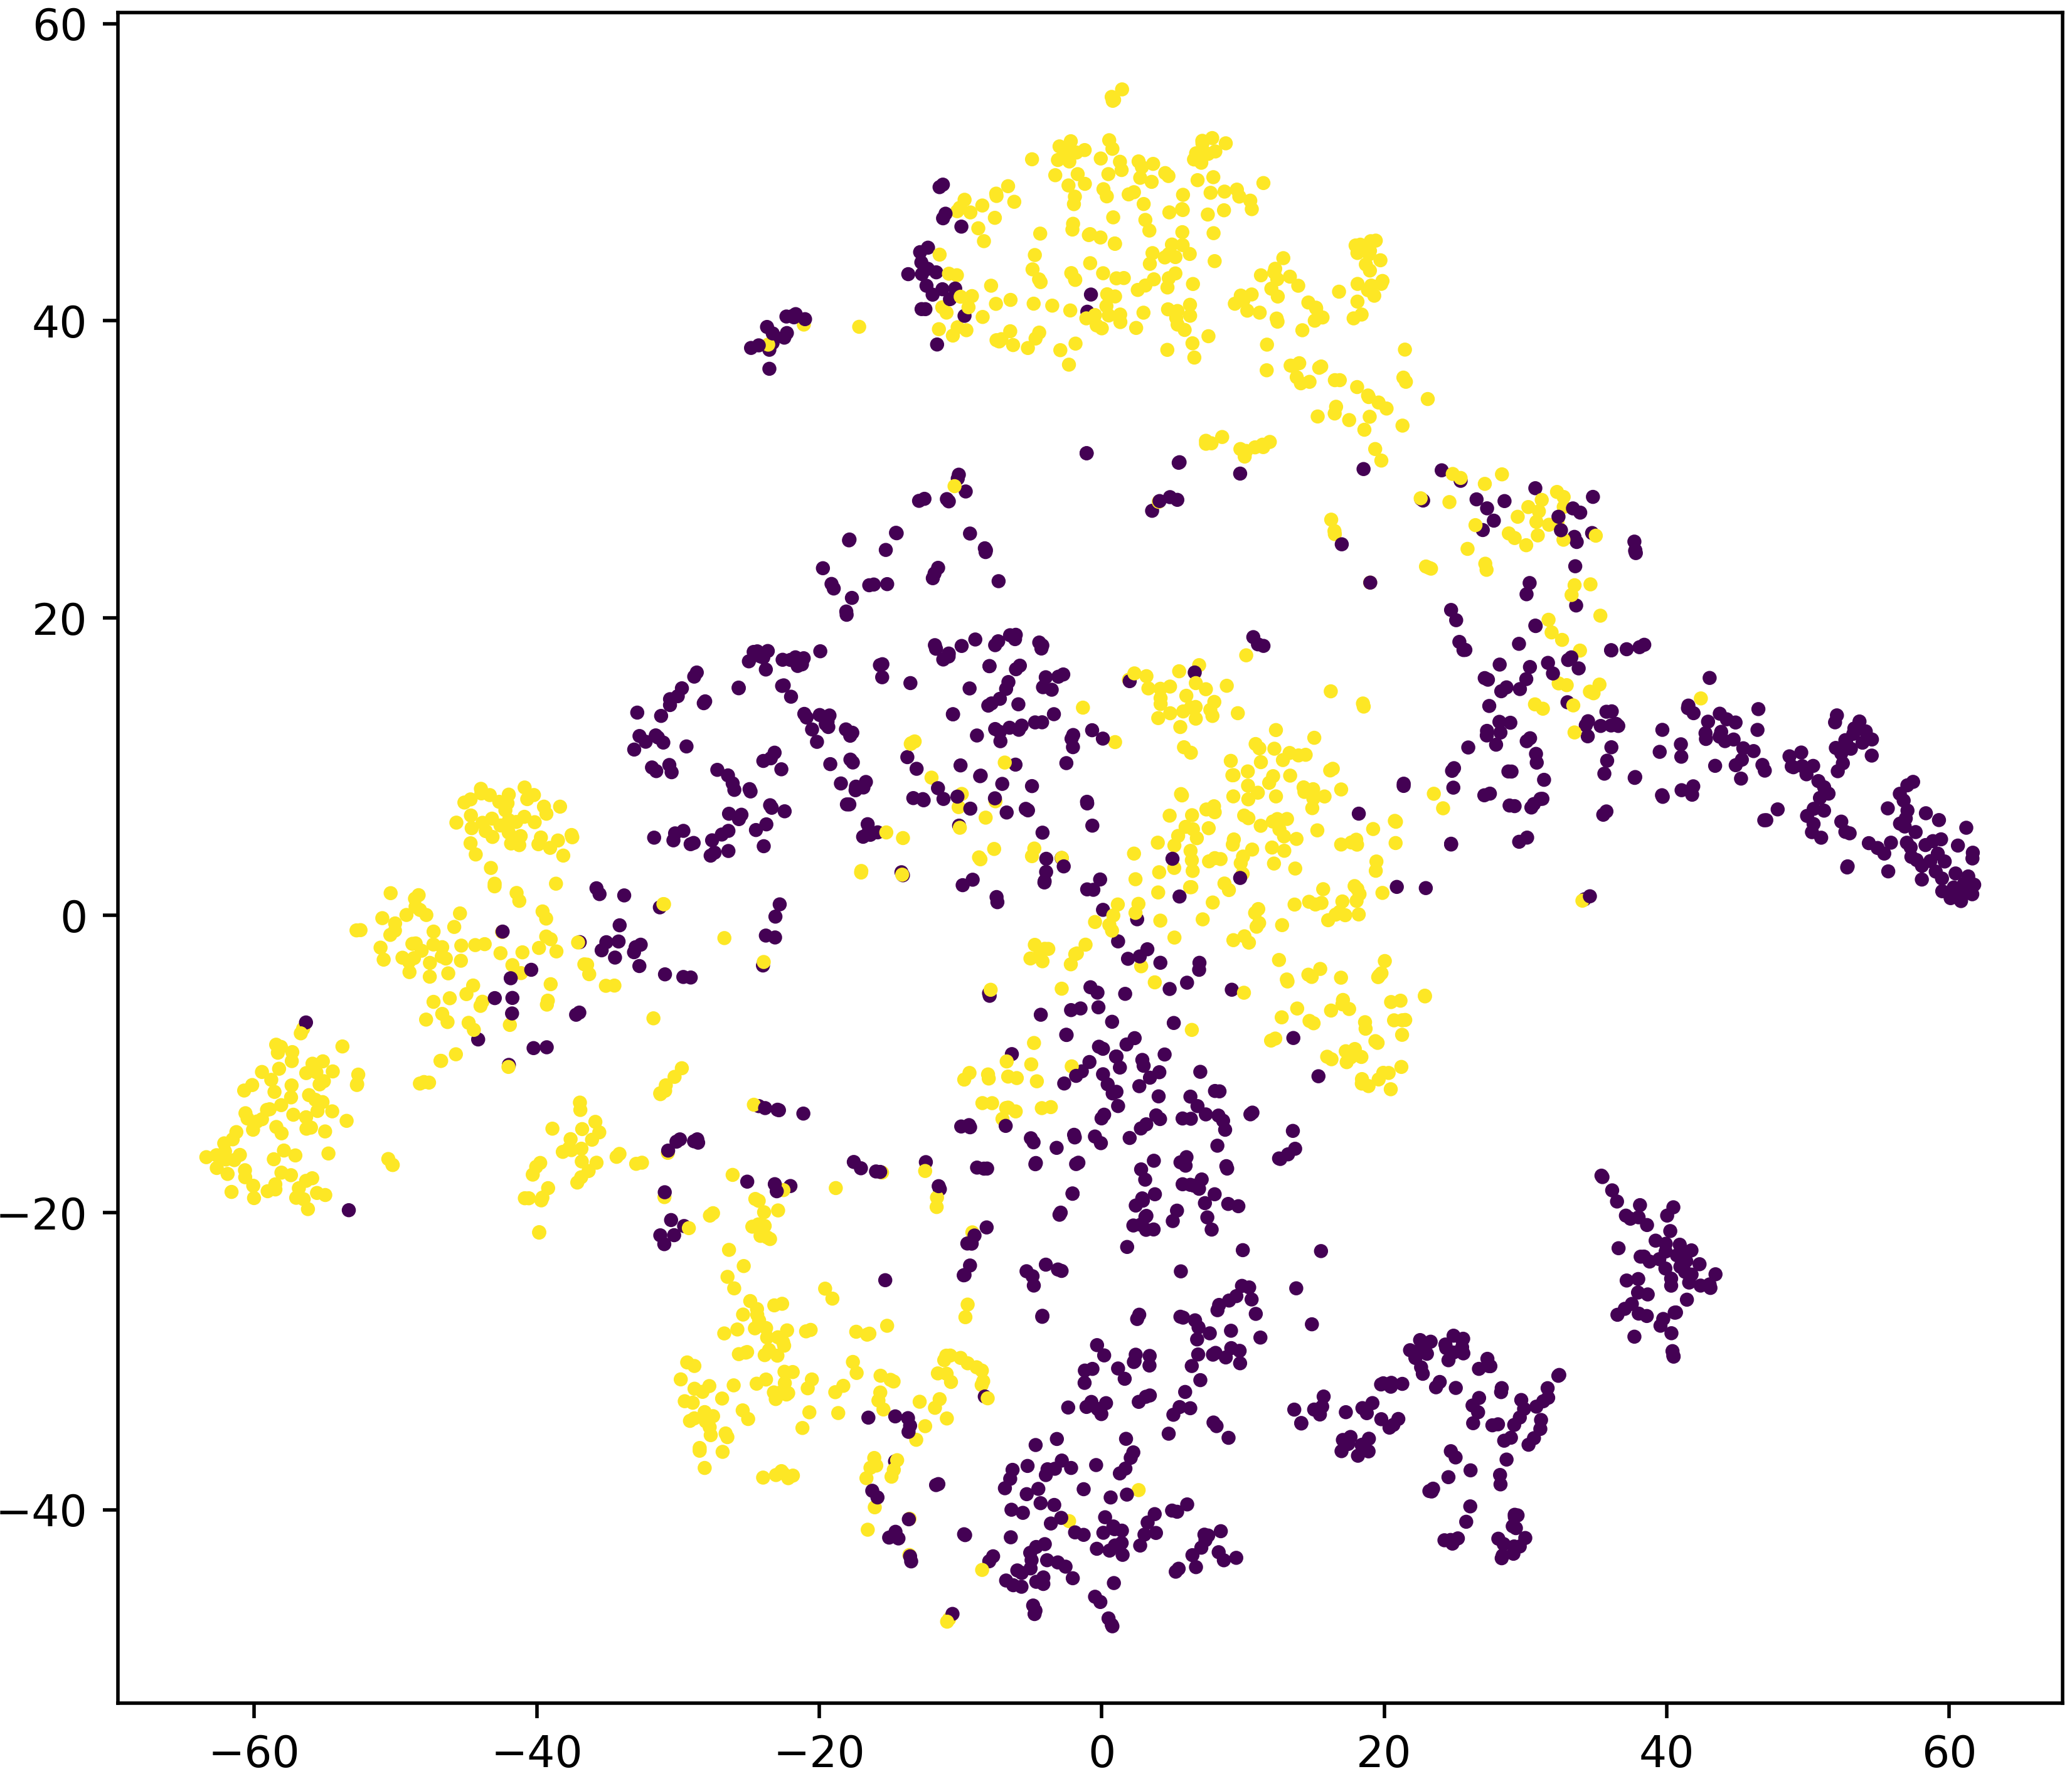
\includegraphics[width=\textwidth]{figure/resnet50_pretrained_tsne.png}
        \caption{Resnet50}
        \label{fig:tsne_resnet}
    \end{subfigure}
    \hfill
    \begin{subfigure}[b]{0.3\textwidth}
        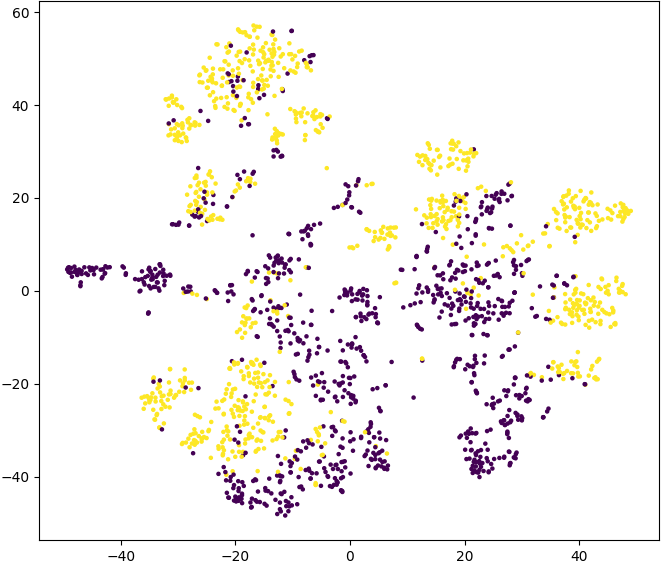
\includegraphics[width=\textwidth]{figure/resnet50_pretrained_finetune_tsne.png}
        \caption{Resnet50 (last layer fine-tune)}
        \label{fig:tsne_resnet_finetuned}
    \end{subfigure}
    
    \hfill

    \vspace{0.5em} % Adjust the space between rows

    \begin{subfigure}[b]{0.3\textwidth}
        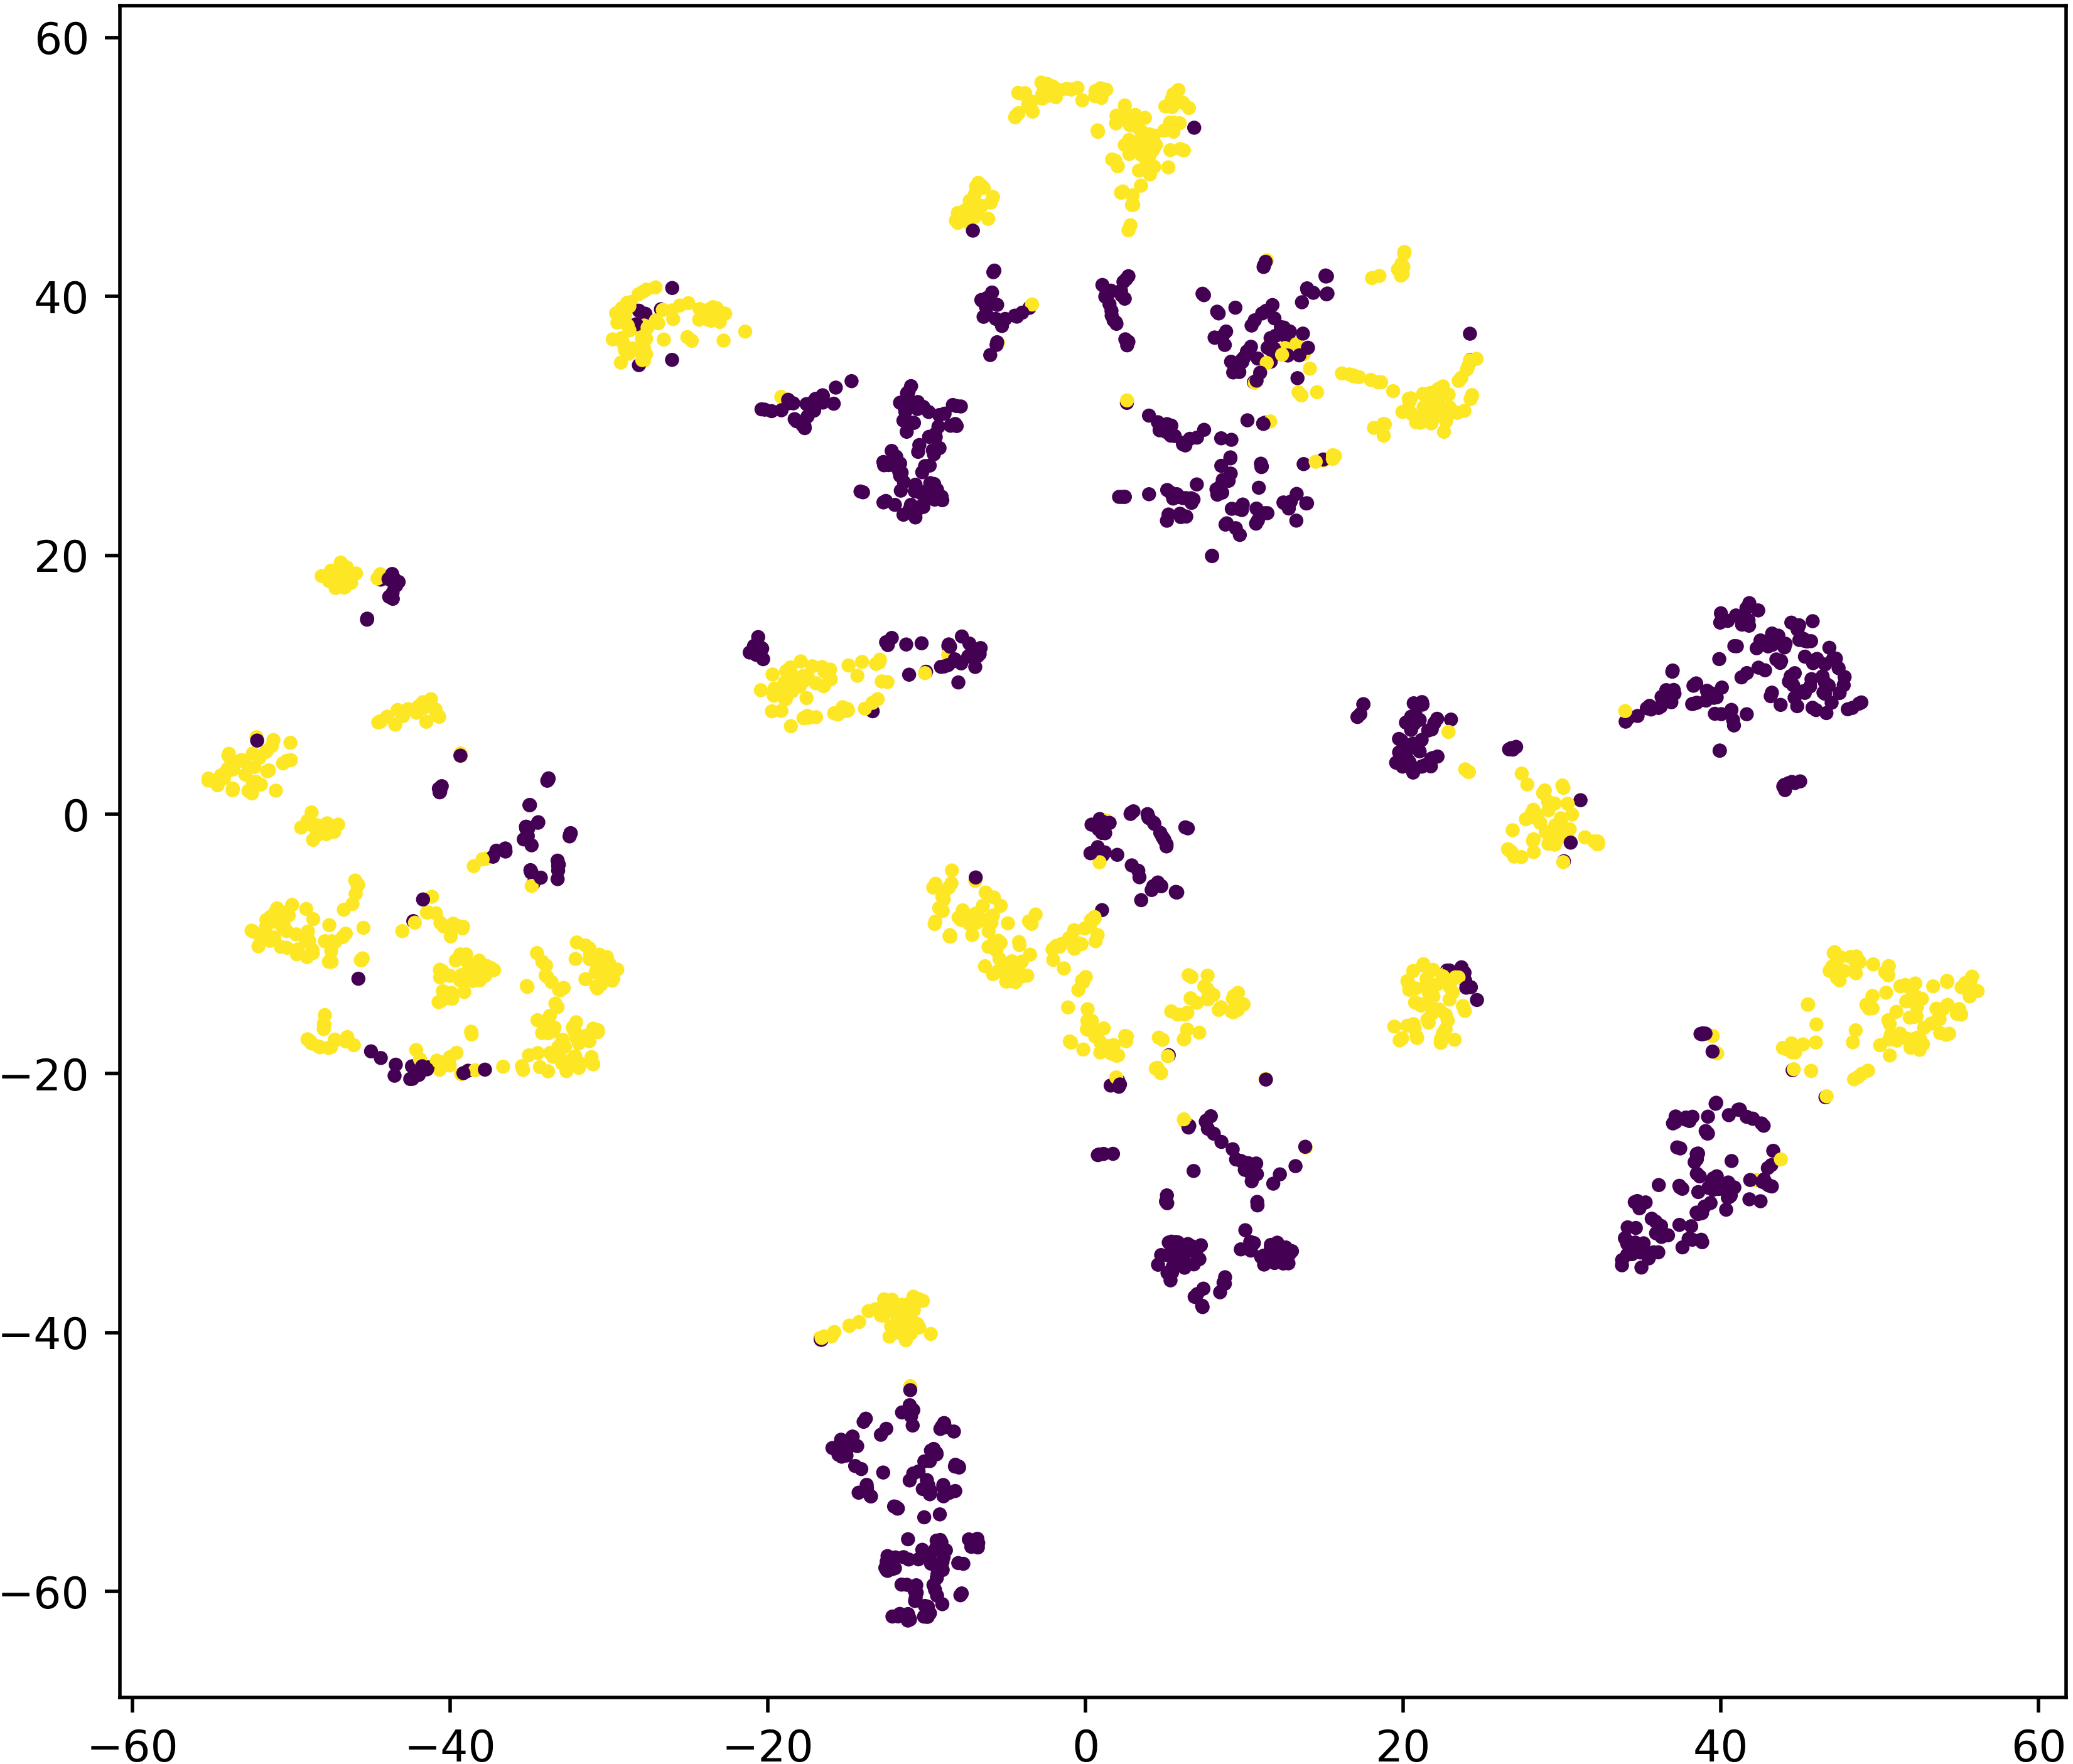
\includegraphics[width=\textwidth]{figure/pathdino_tsne.png}
        \caption{PathDino}
        \label{fig:tsne_pathdino}
    \end{subfigure}
    \hfill
    \begin{subfigure}[b]{0.3\textwidth}
        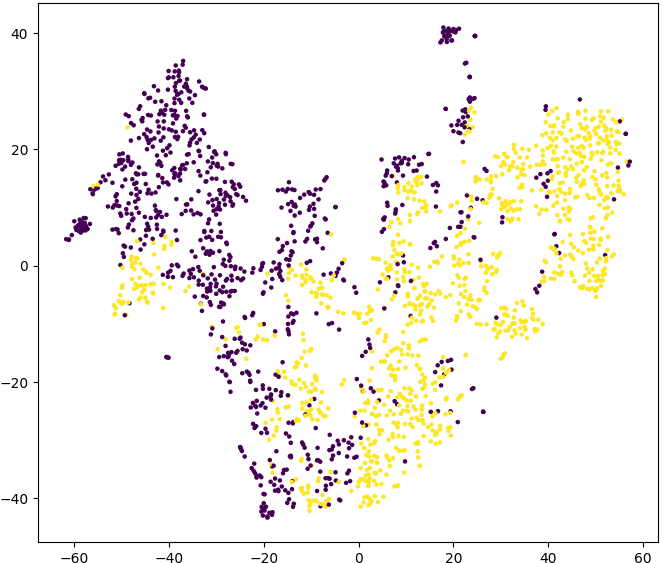
\includegraphics[width=\textwidth]{figure/pathdino_finetuned_tsne.png}
        \caption{PathDino (complete fine-tune)}
        \label{fig:tsne_pathdino_complete_finetune}
    \end{subfigure}
    \hfill
    \begin{subfigure}[b]{0.3\textwidth}
        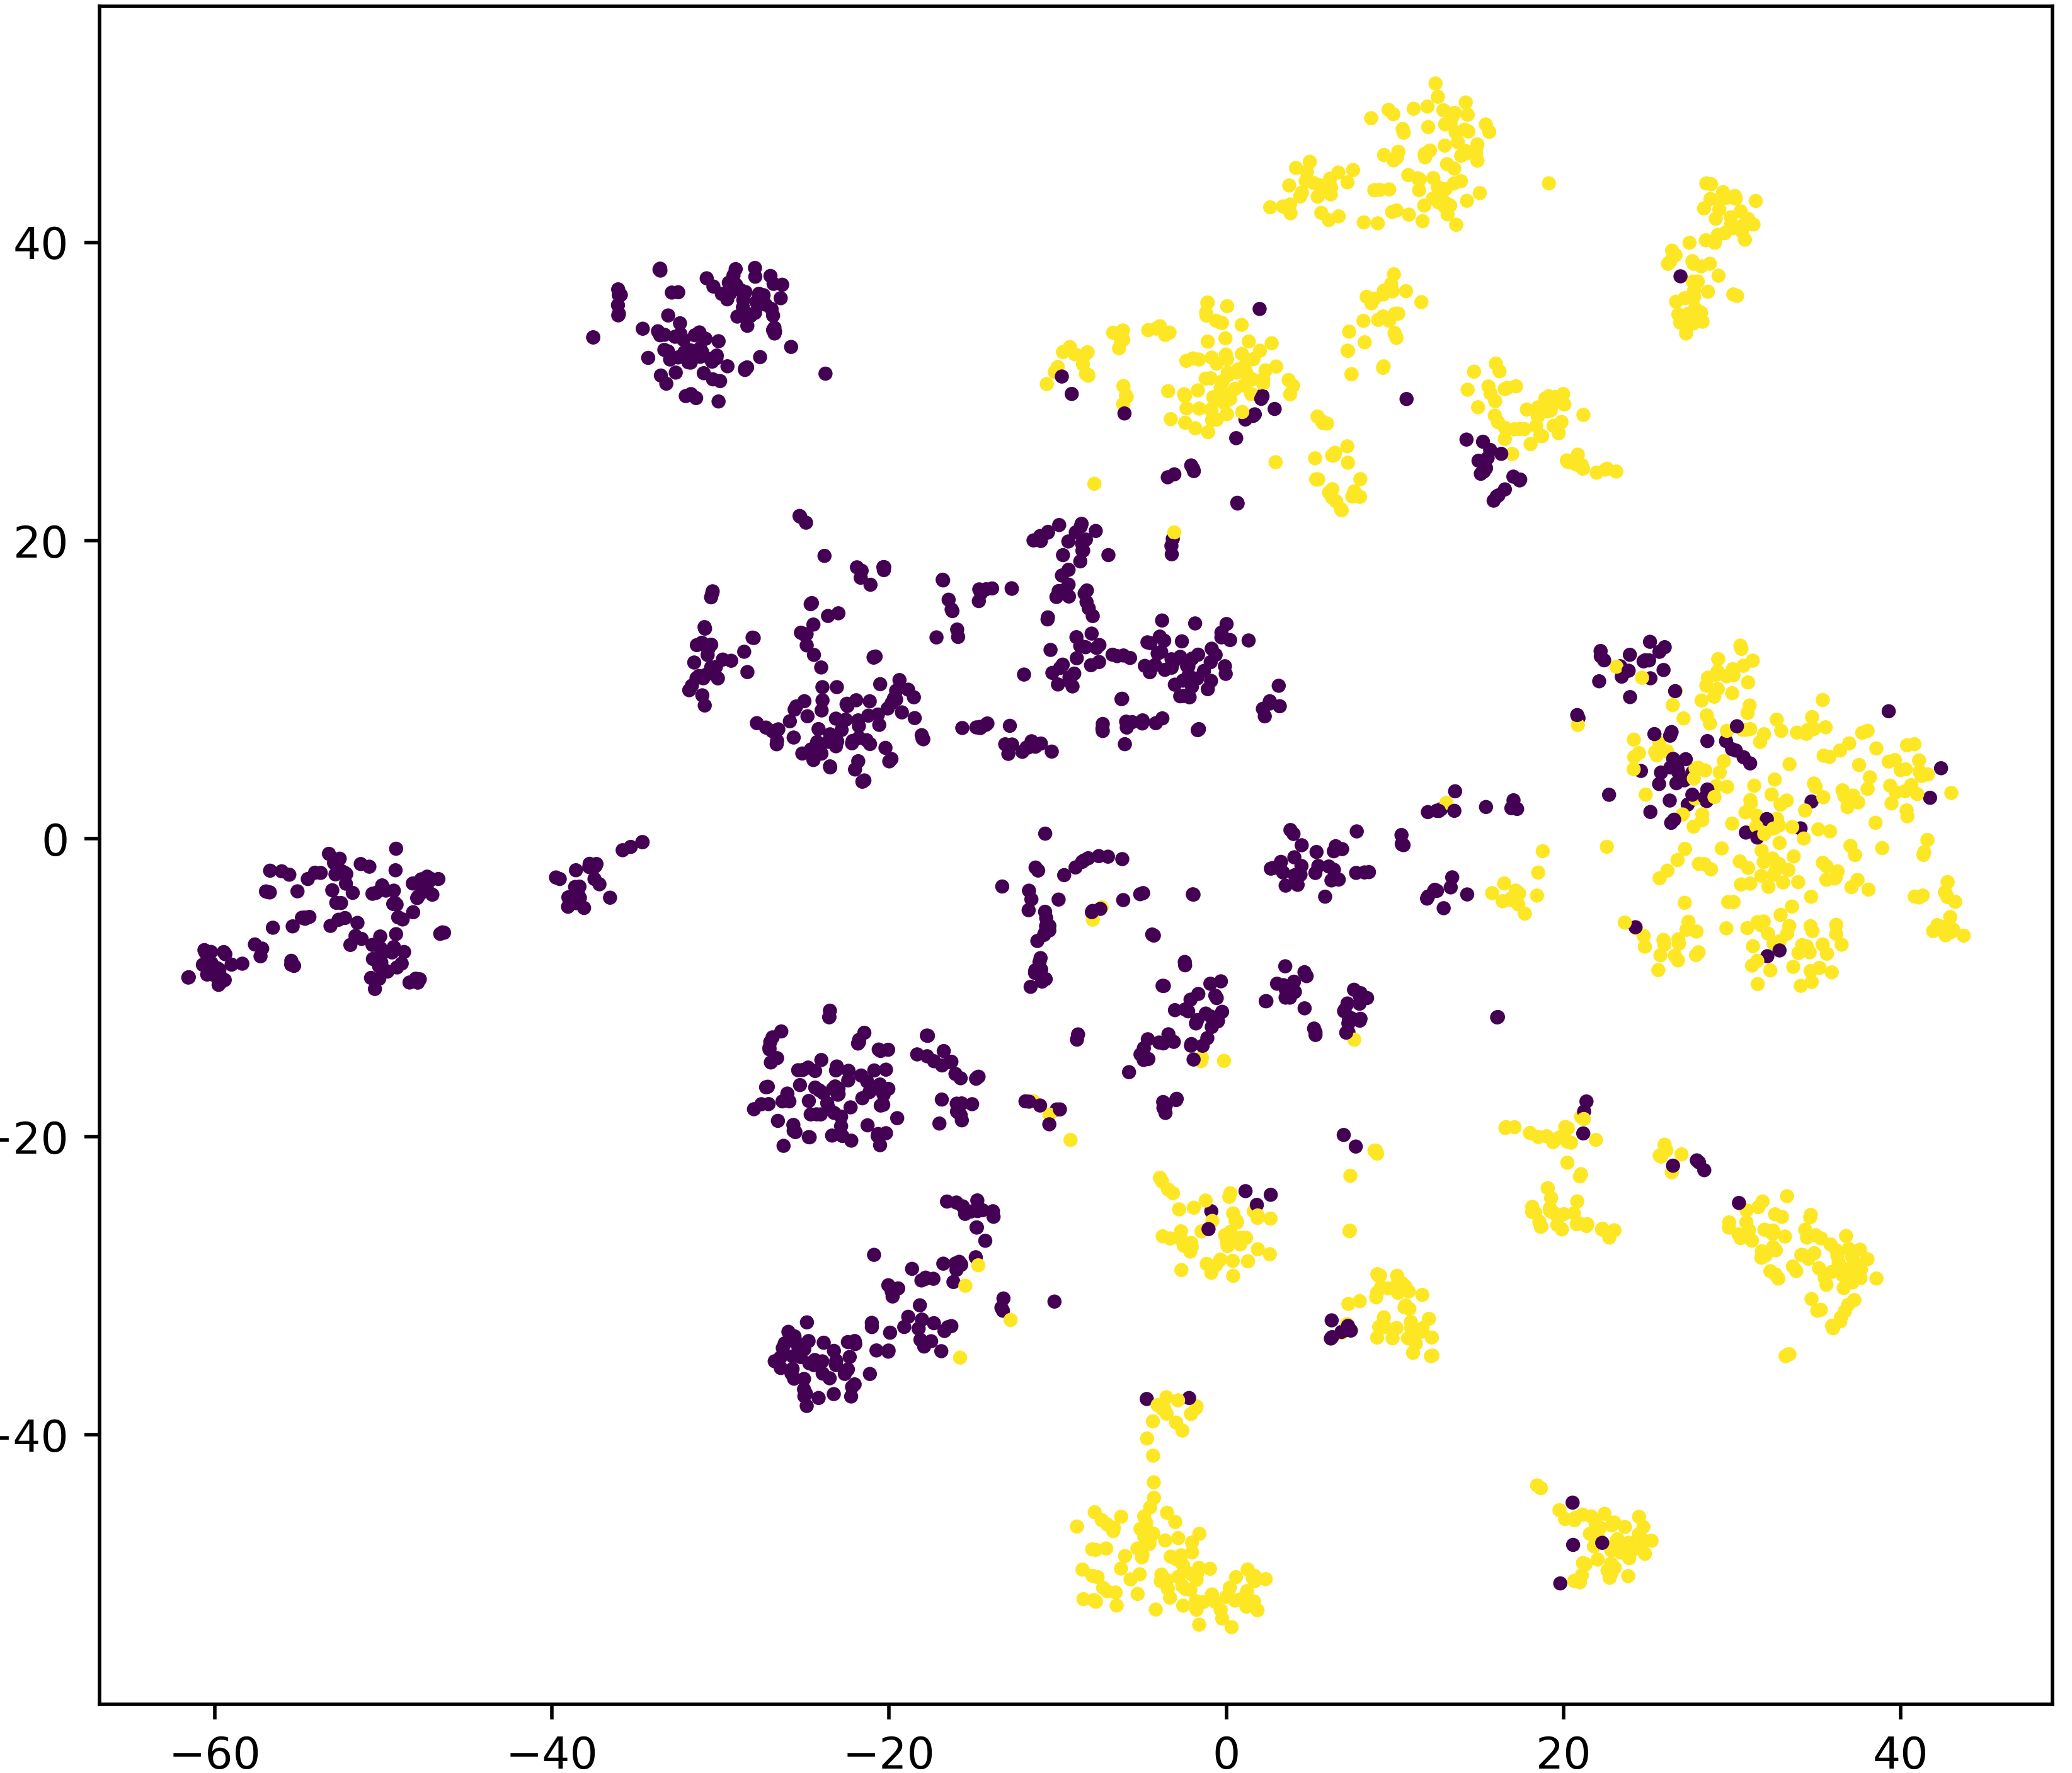
\includegraphics[width=\textwidth]{figure/pathdino_last_layer_finetune_tsne.png}
        \caption{PathDino (last layer fine-tune)}
        \label{fig:tsne_pathdino_last_layer_finetune}
    \end{subfigure}

    \hfill

    \vspace{0.5em} % Adjust the space between rows
    \hfill
    \begin{subfigure}[b]{0.3\textwidth}
        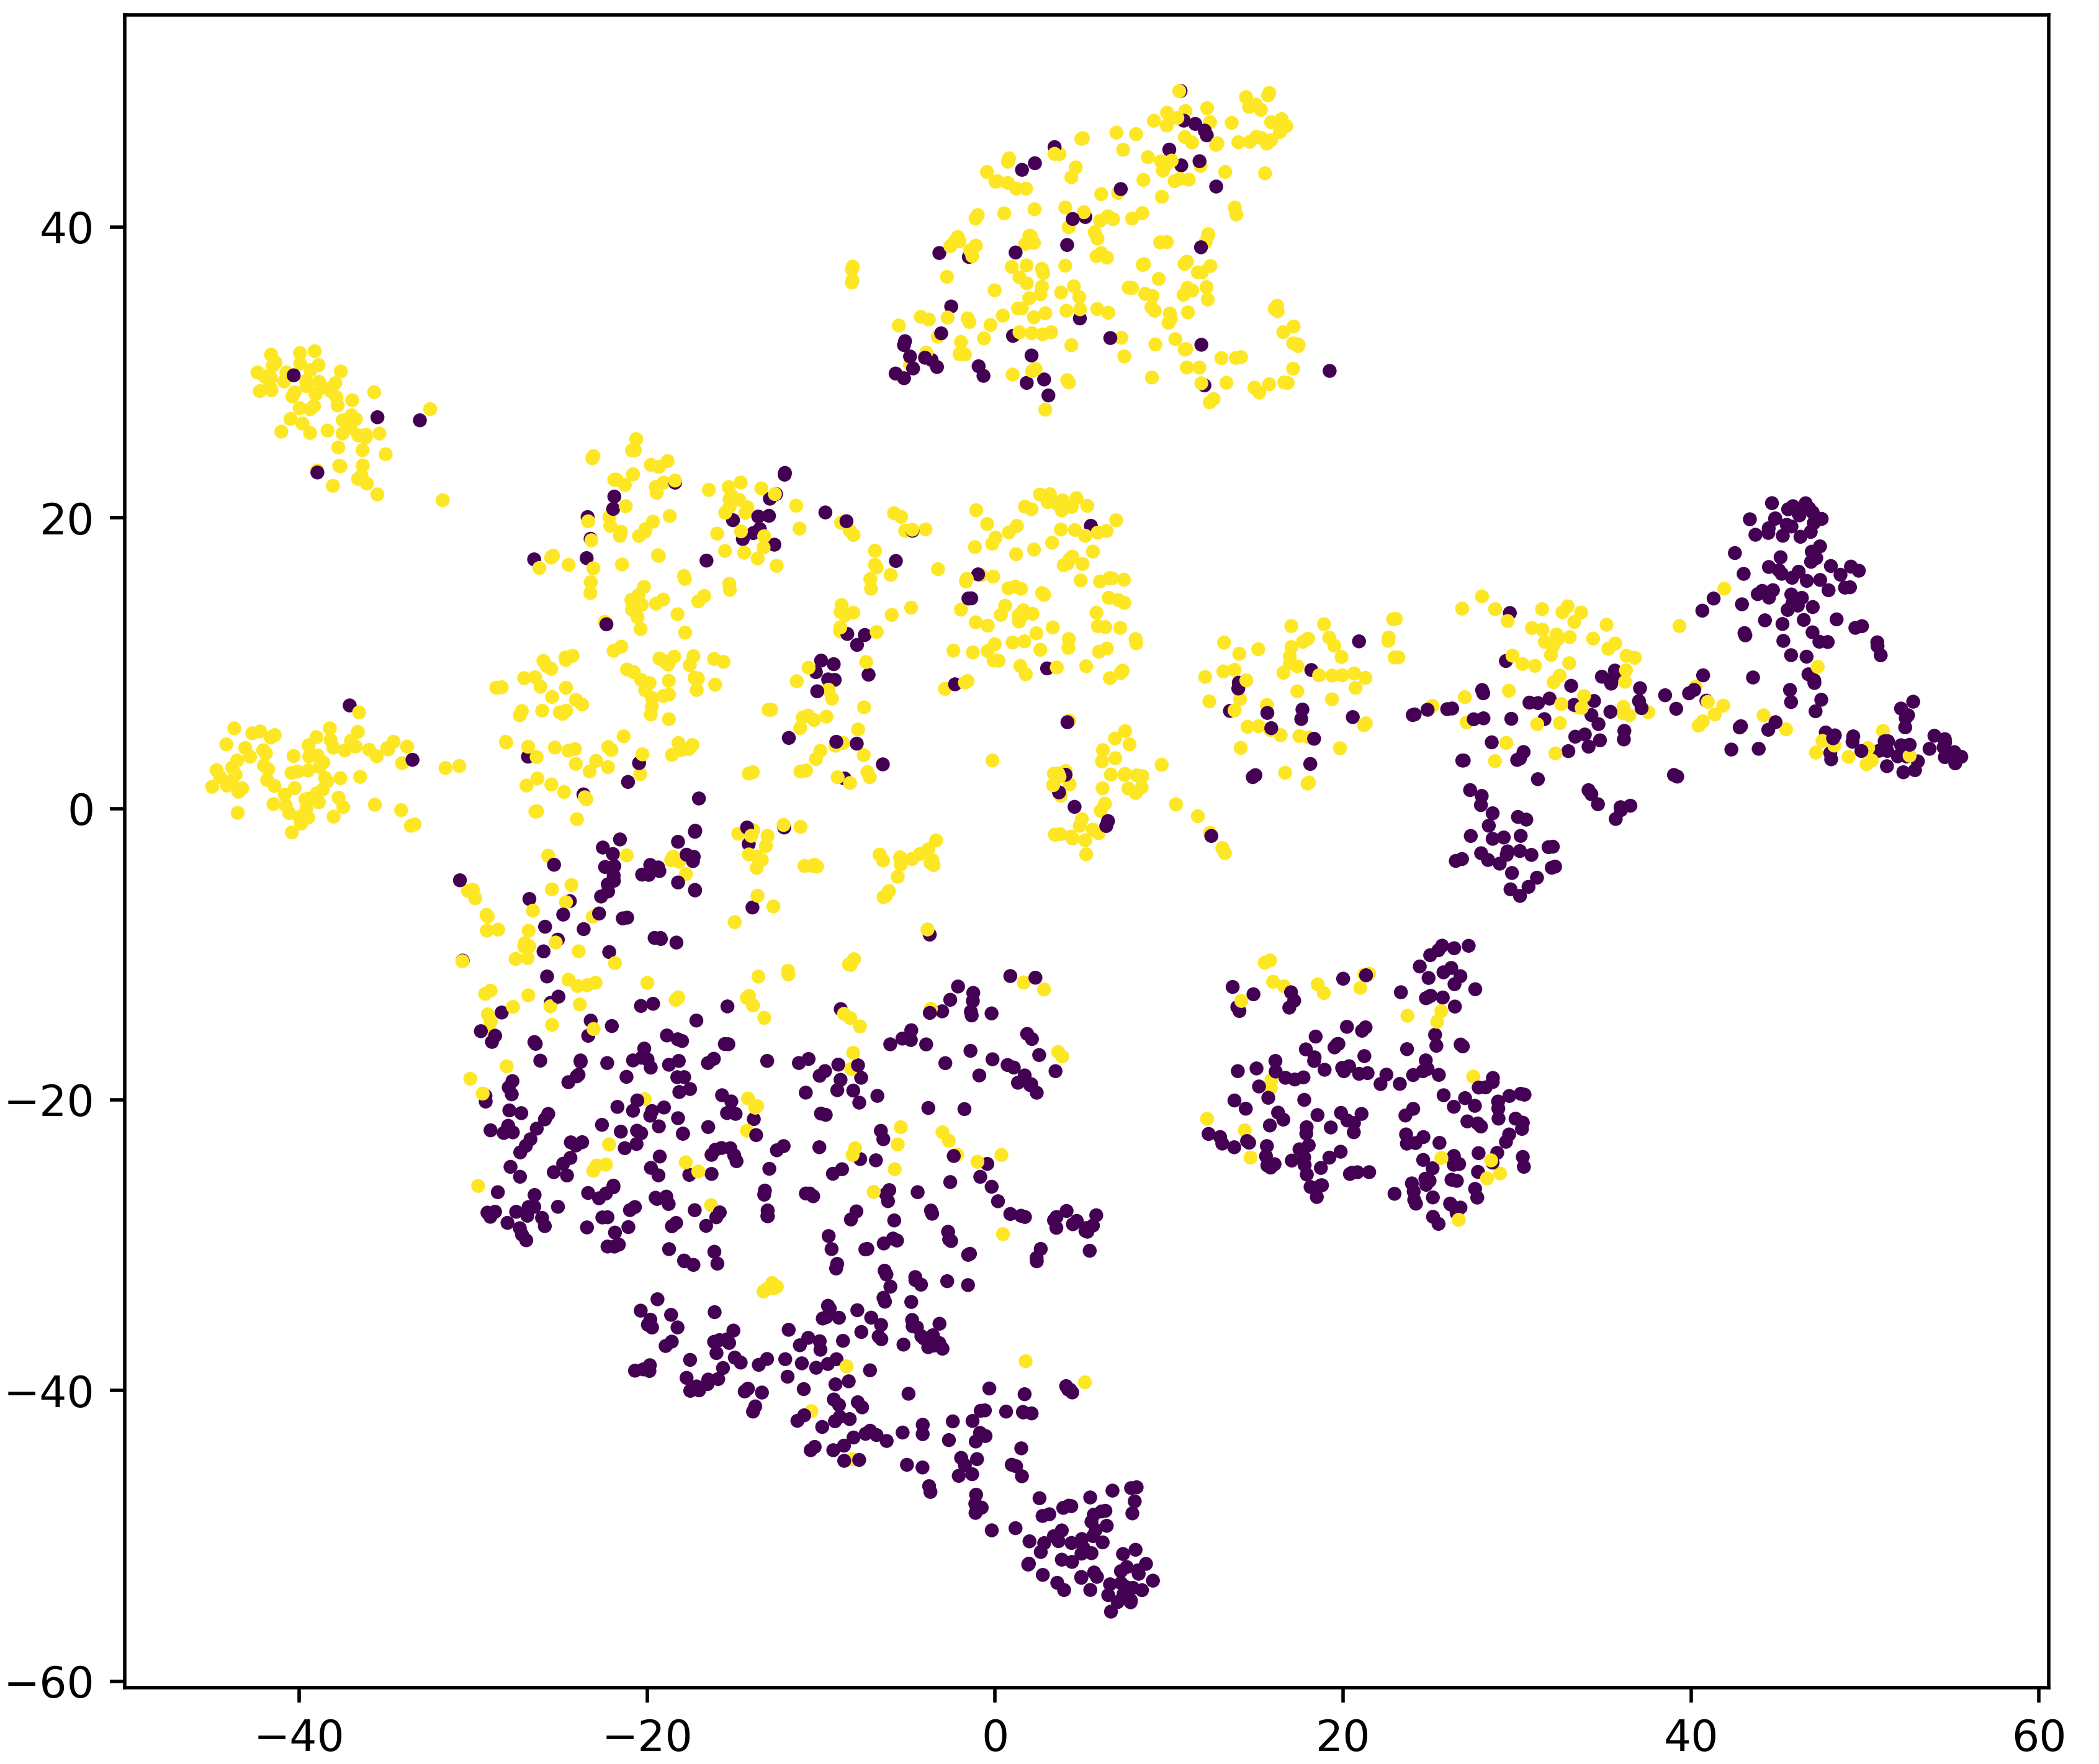
\includegraphics[width=\textwidth]{figure/BYOL_tsne.png}
        \caption{BYOL}
        \label{fig:tsne_byol}
    \end{subfigure}
    \hfill
    \begin{subfigure}[b]{0.3\textwidth}
        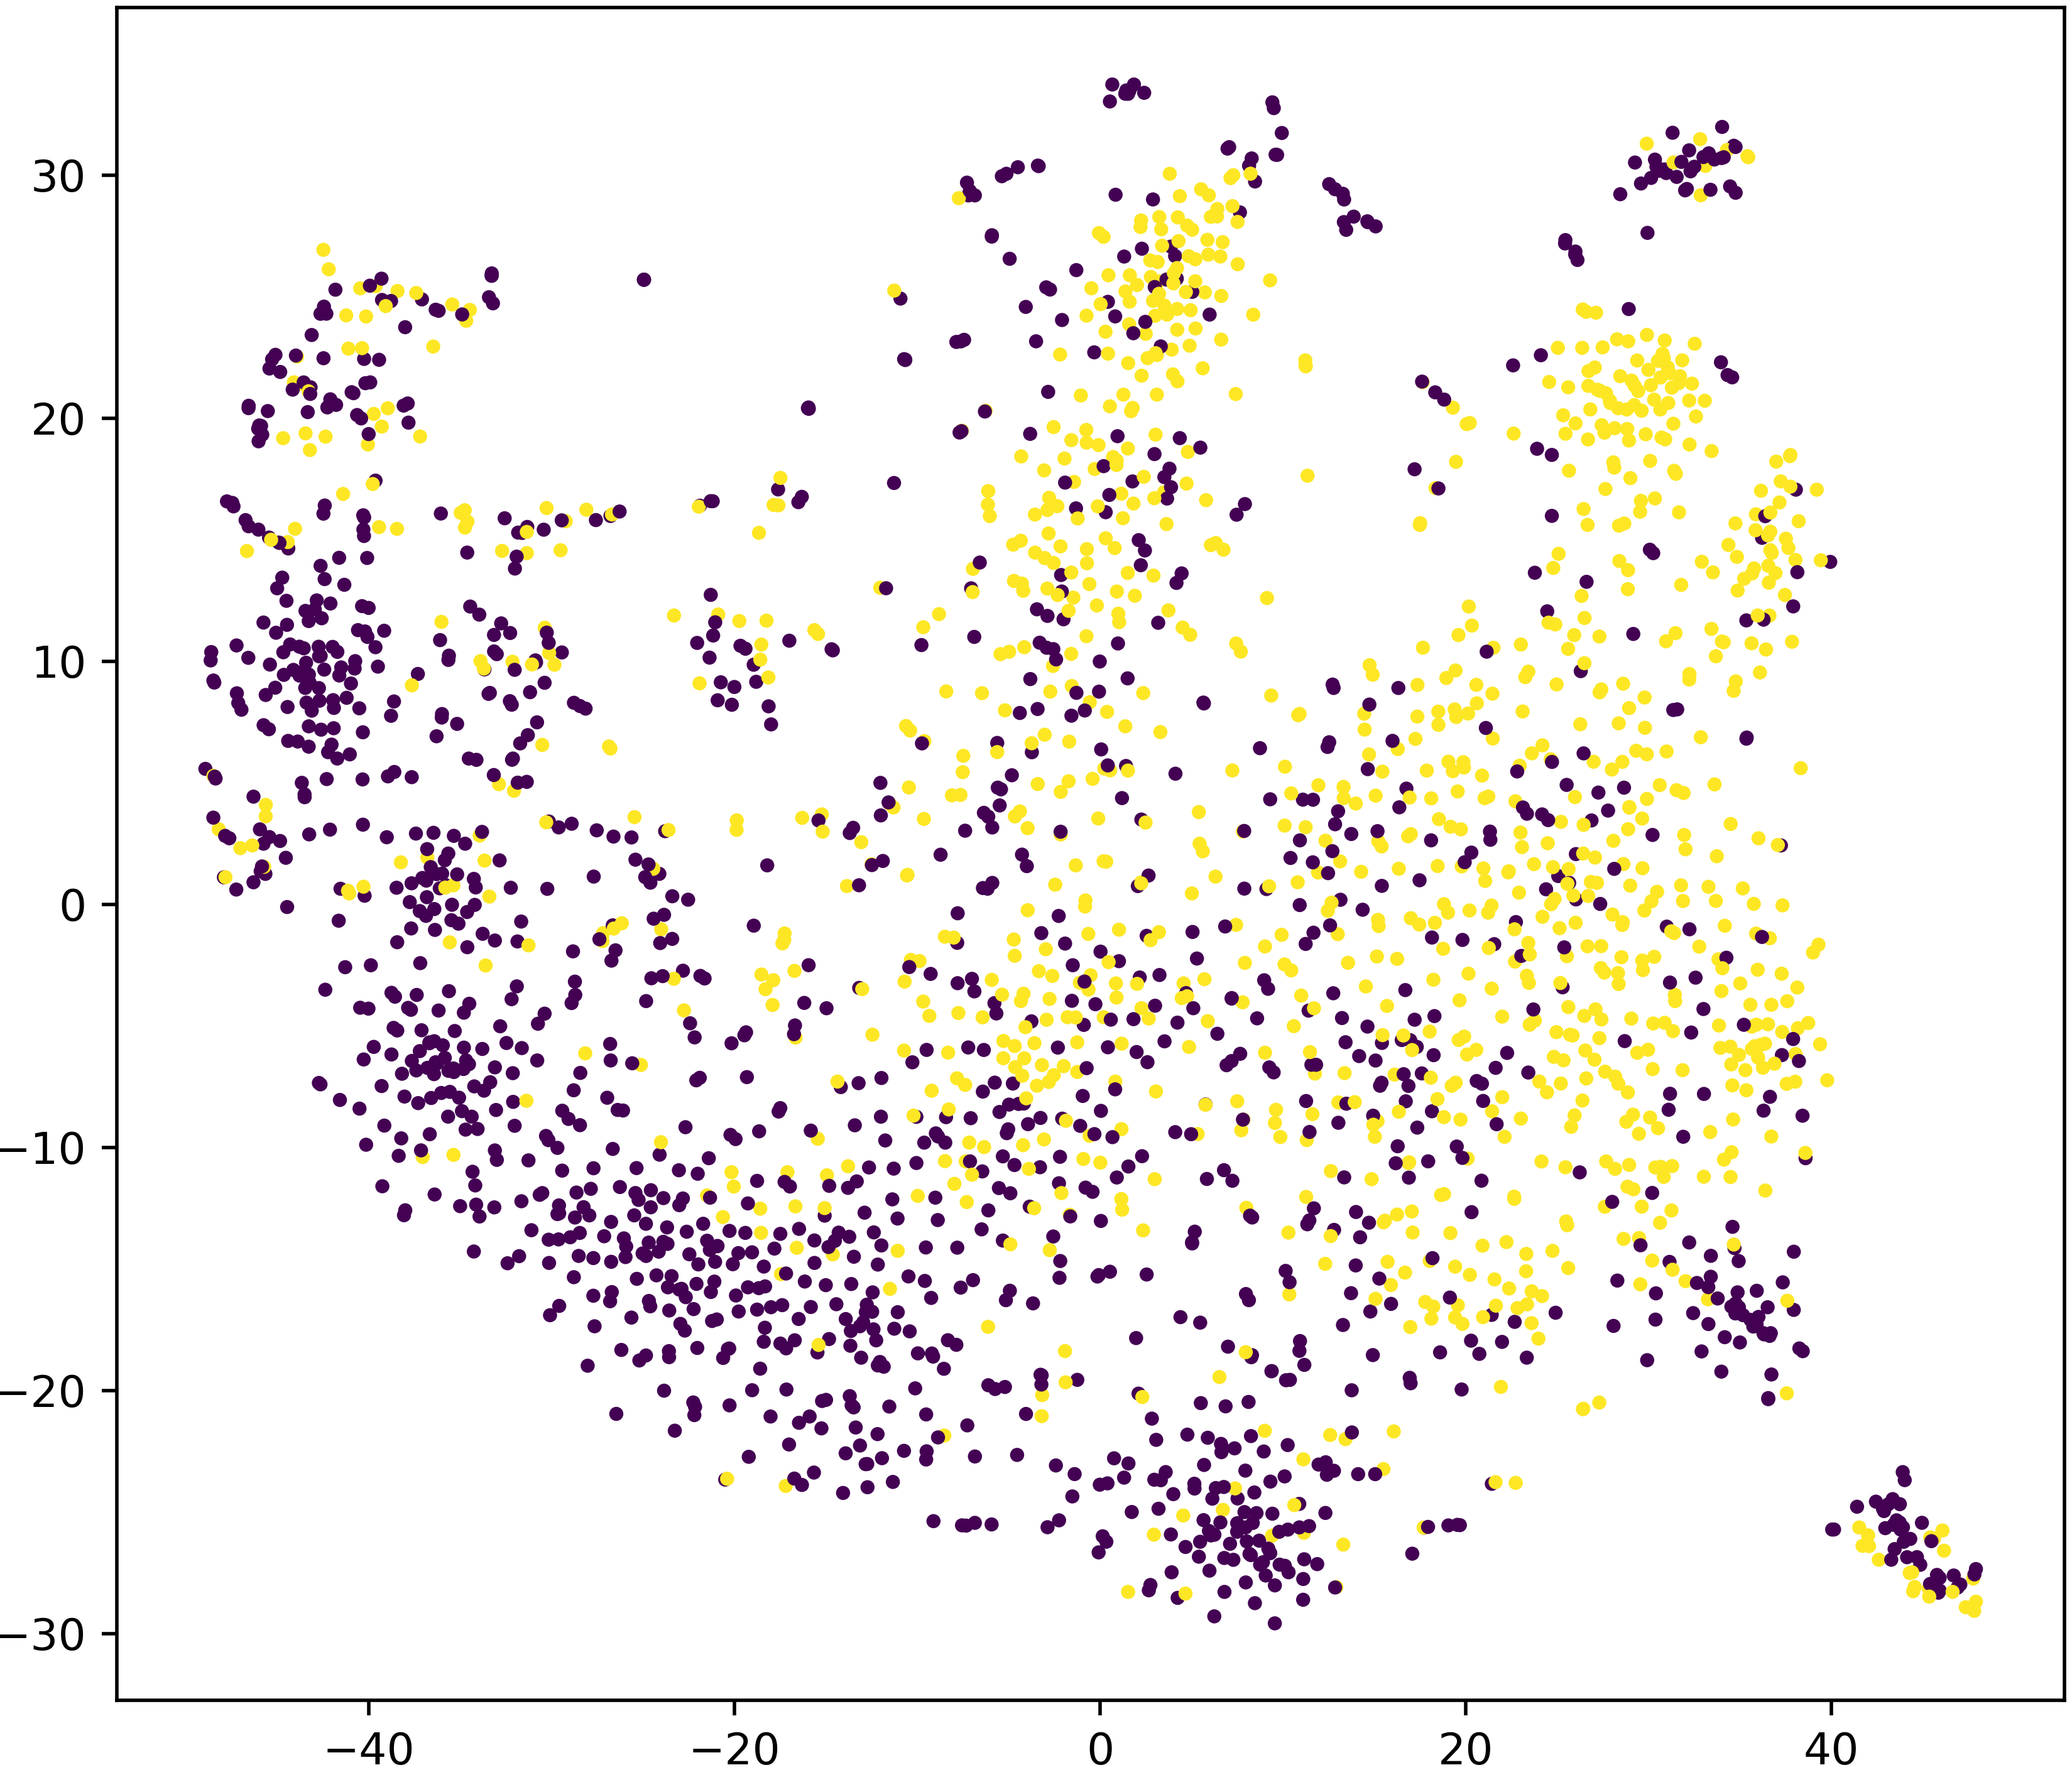
\includegraphics[width=\textwidth]{figure/tsne_resvae.png}
        \caption{ResVAE}
        \label{fig:tsne_resvae}
    \end{subfigure}
    \hfill 
    \hfill

    \caption{ \small t-SNE visualizations for the different methods. These plots show the structure and separation of the latent space learned by our extraction models. Coherently with the numerical evaluation, the t-SNEs reported here show that the original PathDino and its fine-tuned version (last layer), are the most efficient in separating the representations of cancerous and non-cancerous images.}
    \label{fig:tsne}
\end{figure*}


\begin{table}[t]
\centering
\begin{tabular}{l c c c}
\toprule
& \multicolumn{3}{c}{Model Performance} \\
\cmidrule(l){2-4}
Model & Accuracy & Precision & Recall \\
\midrule
Densenet121 (baseline) & 0.78 & 0.78 & 0.78 \\
ResNet50 (baseline) & 0.86 & 0.87 & 0.86 \\
\midrule
ResNet50 (last layer fine-tune) & 0.85 & 0.85 & 0.85 \\
PathDino (last layer fine-tune) & \textbf{0.93} & \textbf{0.93} & \textbf{0.93} \\
PathDino (complete fine-tune) & 0.84 & 0.85 & 0.85 \\
PathDino & 0.89 & 0.89 & 0.90 \\
BYOL & 0.88 & 0.88 & 0.88 \\
ResVAE & 0.75 & 0.74 & 0.74 \\
\midrule
\bottomrule
\end{tabular}
\smallskip 
\caption{\small Models accuracy and macro average precision and recall.}
\label{tab:performance}
\end{table}

\label{sec:results}
In this section, we present and analyze the performance of tested models, as well as the parameters and configurations used to train and evaluate them,
\subsection{Parameters and experiments}
\begin{itemize}


\item \textbf{Baselines}: 
To benchmark the SSL methods fairly, we employed two main strategies. The first is to compare pre-trained models with pre-trained baselines, the second consists in fine-tuning both models and baselines with different tuning depths. This way we provide a comparative understanding of how well models pre-trained on natural images perform on histopathological data, both with and without task-specific fine-tuning. For DenseNet121, we used no tuning strategy, evaluating only the features extracted from the pre-trained model. For Resnet50, we tested features extracted with the pre-trained model as well as with the fine-tuned model. For the fine-tuning setting, we performed both tuning through the entire network and only on the last fully connected layer. All the tuning experiments were conducted for 10 epochs with the same pre-training optimizer and a learning rate smaller than the one used for pre-training. Finally, we used a cosine annealing scheduling with a weight decay of 0.01.


\item \textbf{BYOL}: For the BYOL model, we utilize a batch size of 32, 30 training epochs, a learning rate of $3^{-5}$, and an image size of 256 pixels. The model is implemented using a ResNet architecture pre-trained on ImageNet, and the optimizer employed for training is Adam. 

The data augmentations applied during training are crucial for learning effective representations. We used transformations inspired by the SimCLR \cite{sfclr}  framework, which has proven effective in self-supervised learning settings. The following transformations were applied:

\begin{itemize}
    \item A color jitter transformation with parameters set to 0.8 for brightness, contrast, and saturation, and 0.2 for hue, using a strength factor of $s = 1$. This augmentation can encourage the model to learn color-invariant features.
    \item A random resized crop to randomly scale and crop the image to the desired size of 256 pixels, with a scale range of (0.2, 1.0). This transformation helps the model learn scale-invariant features by presenting objects at different sizes and positions.
    \item A random horizontal flip to flip the image horizontally with a 50\% probability, in order to help the model to be invariant to orientation.
    \item A random Gaussian blur with a kernel size proportional to the image size (computed as $\frac{\text{IMAGE\_SIZE}}{20*2}+ 1$) and a standard deviation in the range of (0.1, 2.0), applied with a probability of 10\%. 
    \item A random grayscale transformation applied with a probability of 20\%. This forces the model to learn features that are not reliant on color information.
    \item A normalization step using mean values of [0.485, 0.456, 0.406] and standard deviations of [0.229, 0.224, 0.225] to match the statistics of the pre-trained ResNet model.
\end{itemize}
We perform two experiments: the first one using all the aforementioned augmentations as they were presented, and the second one where we better adapt them to our WSI scenario. We remove the Gaussian blur augmentation because, while it can help the network to focus on more relevant objects and shapes in natural images, in the context of medical patches, it risks erasing potentially significant details. Finally, in the second experiment, we replace the mean and normalization values of the normalization steps with those computed from our datasets. The second experiment, while it does not drastically change the results, allows us to improve the performance of BYOL by 2\% with respect to its standard version. The results in Table \ref{tab:performance} already show the improved BYOL performance with the updated augmentations. These transformations, implemented using Kornia's augmentation library, are applied twice to generate two different augmented views of the same image, denoted as \texttt{transform1} and \texttt{transform2}. 

\item \textbf{PathDino}: the original PathDino-512 from \cite{pathdino} is trained using around 6 million patches from The Cancer Genome Atlas (TCGA, \cite{weinstein2013cancer}), a batch size of 192, AdamW optimizer and a learning rate of $5^{-4}$ for 27 epochs. For our work, we perform two fine-tuning experiments: one modifying the weights of the entire network, and one freezing everything but the last ViT block. Our fine-tuning is performed for 10 epochs with the same optimizer and a learning rate smaller than the one used for its pre-training (0.0001 instead of 0.0005). Finally, we used a cosine annealing scheduling with a weight decay of 0.01. Note that this setting fairly compares to fine-tuning strategies applied for the Resnet50 baseline.
    

\item \textbf{ResVAE}: our variational autoencoder was trained for 30 epochs with a learning rate of $1^{-5}$, Adam optimizer, a \textit{beta} parameter to weight the KLD loss of $1^{-5}$ and it supports a latent dimension of 128 with an input image of 256x256 pixels.
\end{itemize}


\subsection{Results}

The main results of our model are shown in Table
\ref{tab:performance}. We choose to evaluate our model using the accuracy and the macro average of precision and recall. To further evaluate the learning efficiency of our models we present their t-SNE, which is used to visually assess how well the models have learned to distinguish between classes by showing the clustering and separation of data points in a two-dimensional space. The t-SNE plots are shown in Figure \ref{fig:tsne}.


\subsection{Discussion}
Our study provides several insights into the efficacy of different methodologies for extracting meaningful representations from colorectal cancer whole slide images (WSIs).

Firstly, the findings substantiate the hypothesis that in this domain, self-supervised learning (SSL) methods surpass traditional transfer learning approaches using convolutional neural networks (CNNs) pre-trained on natural images. This is evidenced by the superior performance of SSL models like PathDino and BYOL compared to pre-trained DenseNet121 and ResNet50. The results indicate that features learned directly from histopathological images are more relevant and effective for cancer detection tasks than those learned from natural images, underscoring the importance of domain-specific feature extraction.

Interestingly, the Variational Autoencoder (VAE) did not follow this trend, exhibiting a lower accuracy (0.75) compared to DenseNet121 (0.78). This underperformance may be attributed to the relatively small size of our dataset and the limited computational resources available. VAEs typically require larger datasets to effectively learn representations, highlighting the challenges of applying such models in resource-constrained settings that are common in medical imaging.

Among the SSL methods evaluated, PathDino, pre-trained on a large dataset of WSIs patches, significantly outperformed both the ImageNet baselines and other SSL methods. This result underscores the critical role of domain-specific pretraining in medical imaging. PathDino's superior performance, achieving an accuracy of 0.89 without fine-tuning and 0.93 with fine-tuning the last ViT block, compared to BYOL's accuracy of 0.88, suggests that its architectural design and pretraining strategy are particularly well-suited for capturing relevant features in histopathological images.

BYOL also demonstrated robust performance. This success is attributable to BYOL's self-supervised learning framework, which allows the model to learn pertinent features directly from the data without relying on negative pairs or explicit labels. The flexibility and robustness of BYOL's approach enable it to effectively capture diverse features from WSIs, even without the domain-specific pretraining that benefits PathDino. The t-SNE visualizations further elucidate these findings; BYOL's representations exhibit clear clustering, effectively distinguishing between cancerous and non-cancerous features. This capability to discern meaningful representations, even in the absence of domain-specific customization, highlights BYOL's potential to generalize across different data domains.

Furthermore, our experiments with BYOL reveal the impact of specific data augmentations on performance. We found that removing Gaussian Blur from the SimCLR and correctly normalizing the images, leads to improved results, with accuracy increasing from 86\% to 88\%. This indicates that certain augmentations, while generally beneficial for SSL, may not always be optimal for all types of histopathological data, and careful selection of augmentations can significantly influence model performance.

The fine-tuning experiments revealed notable patterns. Fine-tuning the entire network was generally detrimental for both the baselines and most SSL methods, likely due to overfitting on the relatively small dataset. However, fine-tuning only the last layers resulted in significant improvements for PathDino, enhancing accuracy from 0.89 to 0.93, while the Resnet50 baseline did not improve in this scenario. This suggests that the features learned by PathDino are highly transferable and require only minor adjustments to adapt to specific tasks, demonstrating the effectiveness of targeted fine-tuning in leveraging pre-trained models in clinical scenarios.

The exceptional performance of PathDino can be attributed to several factors. The Fast Patch Selection (FPS) method employed for its training likely facilitates efficient and representative sampling of the WSIs, which is crucial when dealing with large images. Furthermore, its pretraining on a substantial WSI dataset enables the model to capture domain-specific features that are highly relevant to the task, enhancing its ability to perform accurately in medical imaging applications.

Lastly, our results partly challenge the prevailing notion in the literature that rotation augmentations are ineffective for self-supervised learning on histological images. The rotation augmentation used in PathDino (HistoRotate) shows significant benefits because it allows the network to learn rotation-invariant representations. This finding further proves that well-designed augmentations tailored to the specific characteristics of histopathological images can enhance the learning of robust representations.

\section{Conclusions and Future Works}
\label{sec:conclusions}
We conducted a comprehensive evaluation of various self-supervised learning (SSL) techniques for feature extraction from Colorectal Cancer Whole Slide Images (CRC-WSIs). The models under consideration, including BYOL, PathDino, and ResVAE, were compared against traditional transfer learning approaches using pre-trained DenseNet121 and ResNet50 architectures. Our findings demonstrate that the PathDino model, particularly when fine-tuned, outperforms other models, indicating its robustness in capturing meaningful features from histopathological images. 

Future work should explore the integration of larger and more diverse datasets to further validate the generalizability of the models tested in this study. It would also be interesting to exploit the Fast Patch Selection and the HistoRotate techniques from the work in \cite{pathdino} in combination with other models and approaches like the contrastive learning that distinguished BYOL. Additionally, domain-specific augmentations, both in the BYOL domain and in other contexts, could enhance performance.

Beyond the current evaluation framework, exploring new downstream tasks, such as the segmentation of cancerous areas or the identification of specific tissue types, could provide additional insights into the utility of these models in clinical settings.

\bibliographystyle{IEEEtran}
% argument is your BibTeX string definitions and bibliography database(s)
\bibliography{IEEEabrv, bib/bibliography}

\end{document}


%--

Background: Related work
Materials and methods: 

%